\documentclass[11pt,twocolumn]{article}

\usepackage[english]{babel}
\usepackage{float}
\usepackage{graphicx}
\graphicspath{ {./Outputs/} }
\usepackage[margin=0.45in]{geometry}
\usepackage{hyperref}

\title{{\textbf{EN2550 Fundamentals of Image Processing and Machine Vision\\Assignment 01}}}
\author{{\Large 180616T P.M.P.H.Somarathne}}

\begin{document}

\maketitle

\section{Point operations and spatial filtering}

\begin{figure}[H]
\center
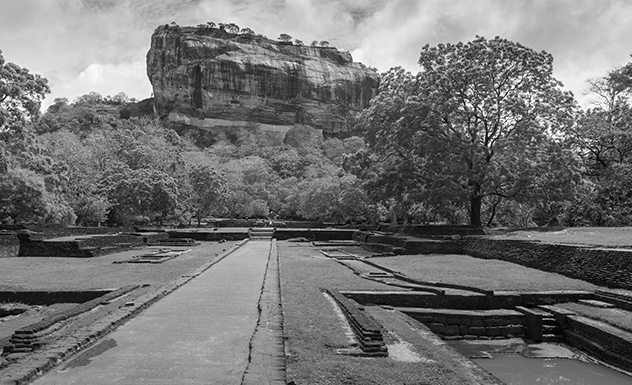
\includegraphics[width=0.25\textwidth]{sigiriya_gray.png}
\caption{{\small \textit{Original image}}}
\end{figure}

\subsection{Histogram equalization}
\begin{figure}[H]
\center
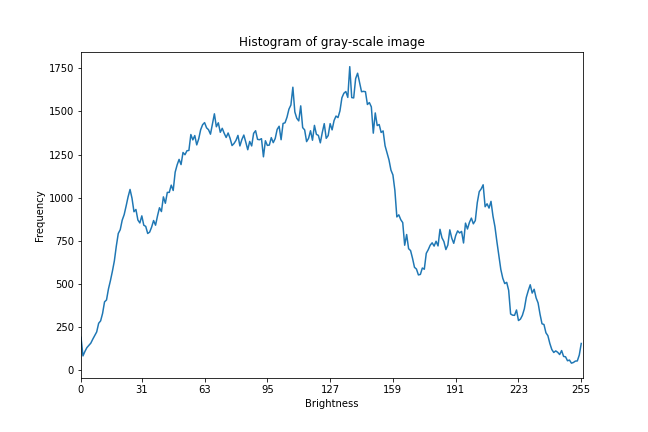
\includegraphics[width=0.3\textwidth]{Histogram.png}
\caption{{\small \textit{Histogram of original image}}}
\end{figure}
\begin{figure}[H]
\center
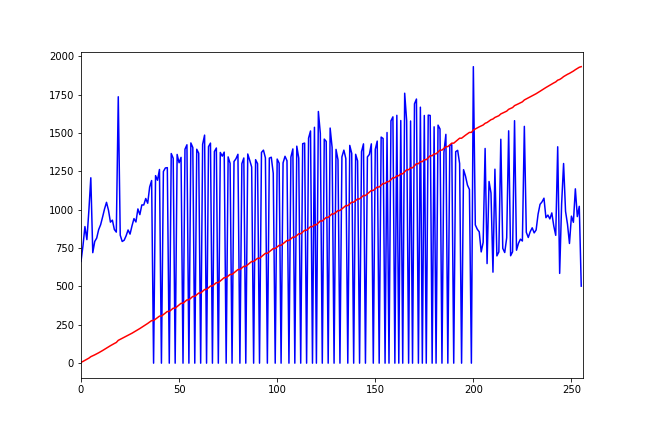
\includegraphics[width=0.3\textwidth]{Equalized_Histogram.png}
\caption{{\small \textit{Equalized histogram(blue) and cumulative(Red)}}}
\end{figure}
\begin{figure}[H]
\center
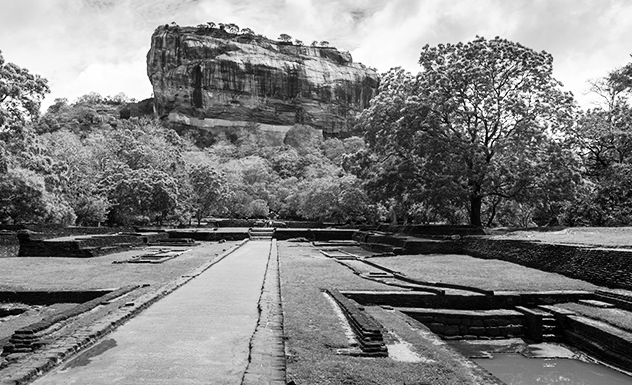
\includegraphics[width=0.25\textwidth]{Equalized_Image.png}
\caption{{\small \textit{Image after equalizing the histogram}}}
\end{figure}


\subsection{Intensity transformations}
\begin{figure}[H]
\center
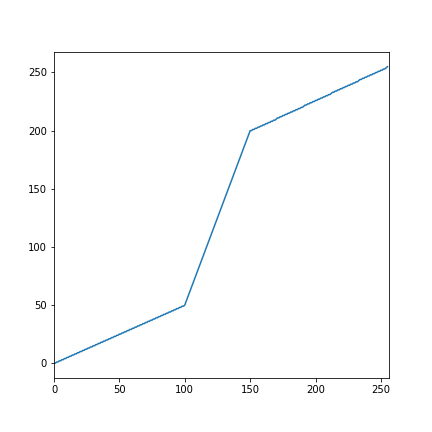
\includegraphics[width=0.3\textwidth]{Intensity_Transform.png}
\caption{{\small \textit{Intensity transform function}}}
\end{figure}
\begin{figure}[H]
\center
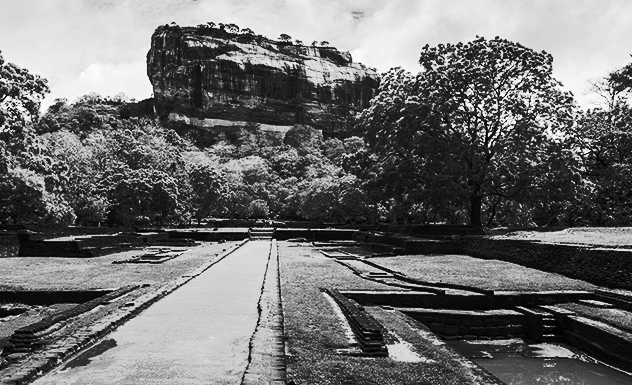
\includegraphics[width=0.25\textwidth]{Intensity_Image.png}
\caption{{\small \textit{Image after applying intensity transform}}}
\end{figure}


\subsection{Gamma correction}
\begin{figure}[H]
\center
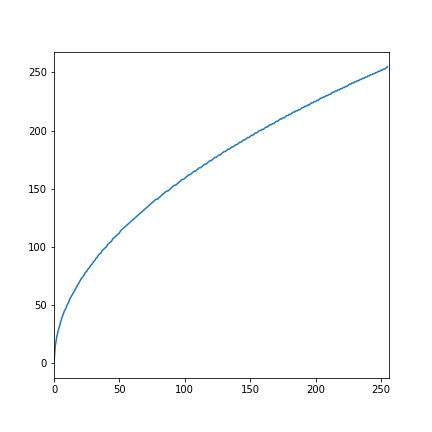
\includegraphics[width=0.3\textwidth]{Gamma_correction.png}
\caption{{\small \textit{Gamma function}}}
\end{figure}
\begin{figure}[H]
\center
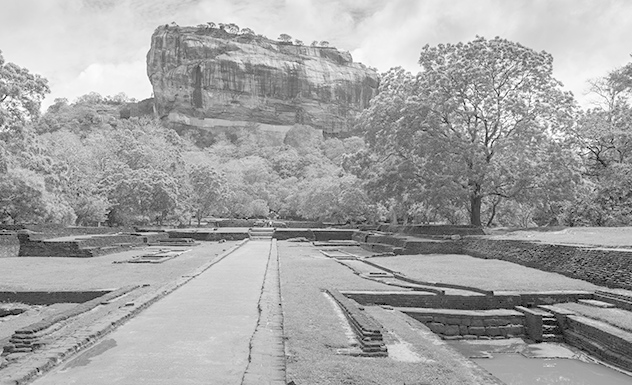
\includegraphics[width=0.25\textwidth]{Gamma_Image.png}
\caption{{\small \textit{Gamma corrected image}}}
\end{figure}


\subsection{Unsharp masking}
\begin{figure}[H]
\center
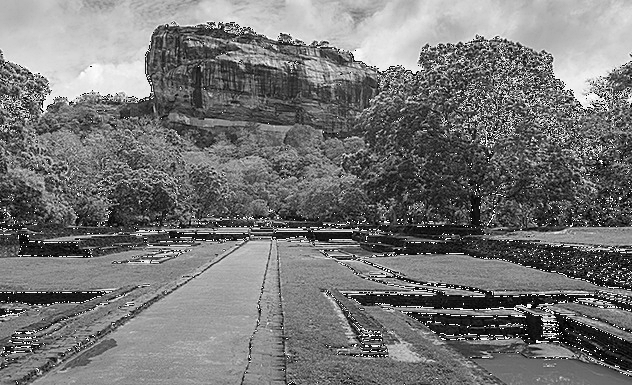
\includegraphics[width=0.25\textwidth]{Unsharp_Image.png}
\caption{{\small \textit{Sharpened image}}}
\end{figure}


\subsection{Gaussian filtering}
\begin{figure}[H]
\center
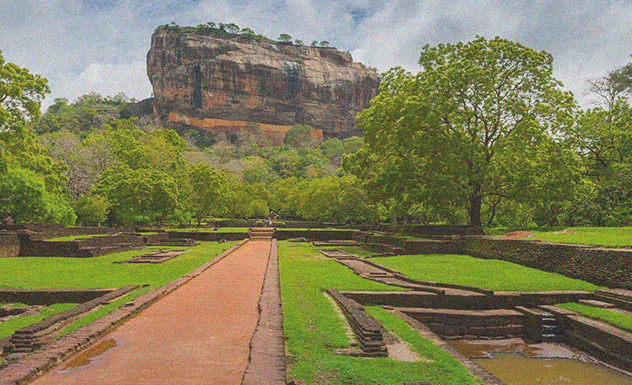
\includegraphics[width=0.25\textwidth]{Noisy_Image.png}
\caption{{\small \textit{Noisy image generated for filtering}}}
\end{figure}
\begin{figure}[H]
\center
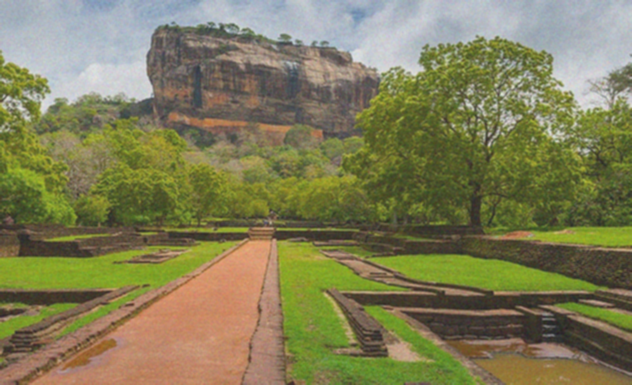
\includegraphics[width=0.25\textwidth]{Gauss_filt_Image.png}
\caption{{\small \textit{Image after applying Gaussian filtering}}}
\end{figure}

\begin{figure}[H]
\center
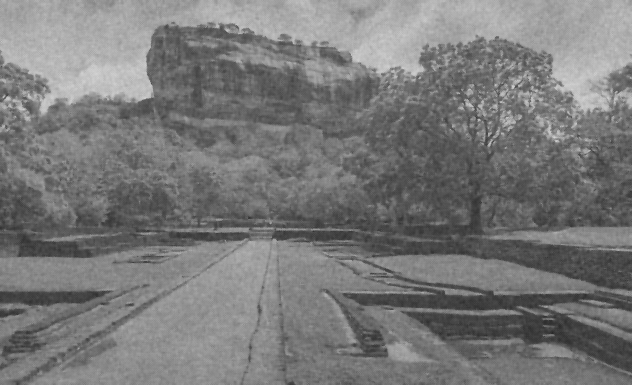
\includegraphics[width=0.25\textwidth]{Bilateral_Image.png}
\caption{{\small \textit{Image after applying bilateral filtering}}}
\end{figure}
\subsection{Bilateral filtering details}


\subsection{Median filtering}
\begin{figure}[H]
\center
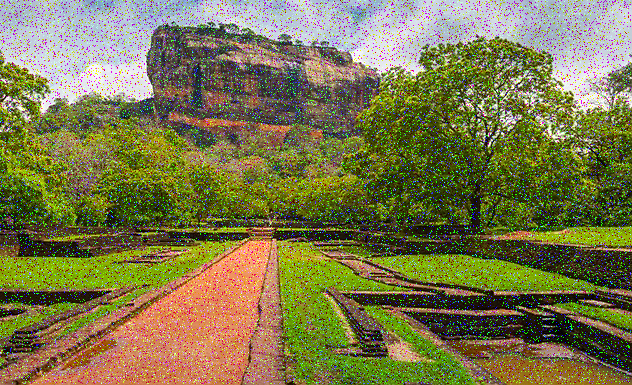
\includegraphics[width=0.25\textwidth]{Salt_Image.png}
\caption{{\small \textit{Image with salt-pepper noise}}}
\end{figure}
\begin{figure}[H]
\center
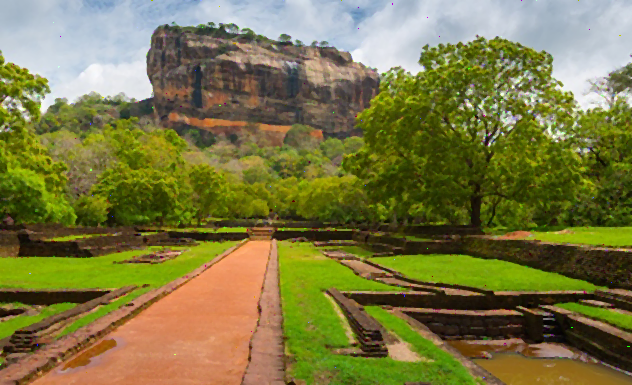
\includegraphics[width=0.25\textwidth]{Median_filt_Image.png}
\caption{{\small \textit{Image after applying median filtering}}}
\end{figure}

\section{Connected component analysis}

\section{Image zooming}


\end{document}